\documentclass[conference]{IEEEtran}
\IEEEoverridecommandlockouts

\usepackage{cite}
\usepackage{amsmath,amssymb,amsfonts}
\usepackage{algorithm}
\usepackage{algpseudocode}
\usepackage{graphicx}
\usepackage{textcomp}
\usepackage{xcolor}
\usepackage{booktabs}
\usepackage{array}
\usepackage{tikz}
\usetikzlibrary{arrows.meta,positioning,fit,backgrounds,shapes.multipart,decorations.pathreplacing}
\usepackage[hidelinks]{hyperref}

\newcolumntype{L}[1]{>{\raggedright\arraybackslash}p{#1}}

\def\BibTeX{{\rm B\kern-.05em{\sc i\kern-.025em b}\kern-.08em
    T\kern-.1667em\lower.7ex\hbox{E}\kern-.125emX}}

\begin{document}

\title{SmartKeyNet: AI-Driven Hybrid Quantum-Classical\\ Key Management for Multi-Tenant Networks}

\author{
\IEEEauthorblockN{Tarun S, Akshay P Shetti, Akshay Nadadhur, Adityaa Kumar H, and Jayashree R}
\IEEEauthorblockA{
Dept. of Computer Science and Engineering (AI \& ML)\\
PES University\\
Bangalore, India\\
taruns0648@gmail.com, akshay190206@gmail.com, akshaynadadhur@gmail.com,\\
adithyakumarh21@gmail.com, jayashree@pes.edu}
}

\maketitle

\begin{abstract}
Cloud key management services are entering a transition in which classical, post-quantum, and quantum-distributed
key material must be served side by side. Quantum key distribution supplies the strongest of the three, but a key pool
that refills at kilobits per second cannot cover every request, so
something has to decide, request by request, who gets what. Static
configuration is the current answer and it fails in both directions:
an always-hybrid rule drains the pool before the requests that
most need it arrive, and fixed thresholds waste quantum material
or withhold it at the wrong moment. We present SmartKeyNet,
a decision layer that treats this as a resource-budgeting problem
for a deep Q-network while keeping security out of the objective
entirely. A threat forecaster and a locked policy table resolve a
minimum protection tier for each request, and every action below
that tier is removed from the action set before the agent evaluates
it. The agent optimizes only latency, energy, key freshness, and
a scarcity price on pool consumption. That separation is the
claim we test: designs placing a threat score inside the reward
can be steered toward weaker key material by an adversary who
shapes that score, whereas masking leaves the same manipulation
able only to raise floors. On a QKD-degradation scenario the
masked agent records zero below-floor decisions against 27,301
for a reward-shaped agent trained on the same environment,
and reaches zero pool-exhaustion events where a tuned threshold
reaches 42. It pays for both in rekey churn, which we report
alongside.
\end{abstract}

\begin{IEEEkeywords}
action masking, adversarial machine learning,
deep reinforcement learning, interpretability, key management,
post-quantum cryptography, quantum key distribution, safe reinforcement learning
\end{IEEEkeywords}

\section{Introduction}

Traffic encrypted with classical public-key cryptography
today can be recorded and stored until a cryptanalytically
relevant quantum computer exists, a threat usually called
harvest-now-decrypt-later~\cite{ref1}. The standardization response is
underway: ML-KEM is a NIST standard~\cite{ref2}, and CNSA 2.0
sets dated migration deadlines for national security systems
\cite{ref3}. What none of it removes is the intermediate period.
For a decade or more, classical, post-quantum, and quantum-distributed key material will coexist inside the same infrastructure, and operators will have to choose among them
continuously.

Quantum key distribution is the awkward member of that
set. Its security argument rests on physics, not computational
hardness, and metro-scale field trials are long established~\cite{ref4},
\cite{ref5}, but the delivered secret-key rate is measured in kilobits
per second and degrades as the quantum bit error rate rises. In
the ETSI GS QKD 014 key-delivery architecture~\cite{ref6}, keys are
drawn from a pool behind a REST interface that refills slowly
and drains at whatever rate consumers ask. A hospital tenant
storing records for thirty years and a logging service retaining
data for six hours both present as key requests to it. Somebody
has to triage, and today that somebody is a configuration file.
The triage is a sequential decision problem with an unusual
property: decisions are coupled, because serving a hybrid key
now is why one may be unavailable in twenty minutes, and a
per-request recommender optimizes each request in isolation
and cannot express that tradeoff at all.

The obvious way to apply reinforcement learning here is
also, we think, the dangerous one. Risk and threat signals
routinely enter RL reward functions in security settings~\cite{ref7},
\cite{ref8}, and folding a threat score in so the agent is paid for choosing stronger cryptography is a reasonable-looking default.
The resulting policy holds security as a preference, weighted
against latency and energy, so an adversary who can influence
the estimator's inputs (for a telemetry-driven estimator, simply
someone who shapes traffic) can bid the security term down.
Input-shaping attacks on learned policies are established~\cite{ref9},
and a reward term is only ever as trustworthy as the signal
feeding it.

SmartKeyNet takes the opposite structure. A threat forecaster and a policy table resolve a minimum protection tier
per request, and the environment deletes every action below
that tier before the deep Q-network sees the action set~\cite{ref10}.
The reward contains latency, energy, key freshness, and a price
on pool consumption --- and no security term, at any weight, at
any point in training. The threat signal can only move floors
upward, so an adversary who convinces the forecaster that
an attack is underway makes the system serve stronger keys
and burn pool faster: an availability cost, not a confidentiality
failure.

Our contributions are: (i) a formulation of hybrid-era key
serving as a masked Markov decision process whose scarce
resource is a QKD pool and whose security requirement is a
constraint rather than an objective term; (ii) a steering-attack
protocol that reproduces a soft-reward baseline and measures,
as a dose-response curve, how far an adversarially shaped threat trace pushes each design below its intended tier; and (iii)
a decision-trace interface exposing the six computed values
behind every action, which the masked design makes possible
and a soft-reward design structurally does not. We are also
explicit about what is built (Section~\ref{sec:impl}): the environment,
the masked agent, the reward-shaped baseline and the four
non-RL baselines run, and the results below come from them.
The learned forecaster and the adversarial trace generator do
not exist yet, so the dose-response sweep of Section~\ref{sec:steering}
remains protocol and not measurement.

\section{Related Work}

Reinforcement learning is by now a standard tool for
adaptive cyber defense, and surveys of the area document
reward functions that carry a risk or threat term alongside
performance objectives~\cite{ref7}, \cite{ref8}. The recurring shape is ``benefit
of security minus cost of security,'' tuned by a weight. We do
not attribute the specific soft-reward configuration we attack to
any single paper. We construct it as a reference design in that
idiom, state the weight we give its security term, and report
how sensitive the attack is to that weight (Section~\ref{sec:steering}); a
steering result that held only at one convenient weight would
not be worth much.

Treating a requirement as something other than a reward
term is not new. Safe reinforcement learning surveys sort the
field into two families~\cite{ref11}: one changes what the agent optimizes, the other changes how it explores. Constrained policy
optimization belongs to the first and enforces expected-cost
limits during training~\cite{ref12}. Those methods bound constraint
violation in expectation, which is the right tool when the
constraint is statistical. Ours is not: a key served below its
policy floor is a discrete compliance event, and an expectation-level guarantee that permits it occasionally is not useful to
an auditor. Invalid action masking gives a per-step guarantee
instead~\cite{ref10}, at the cost of requiring the constraint to be
computable before the action is taken. Here it is: the floor
is a table lookup on sensitivity class and current posture.

Learned policies can be attacked through their observations
\cite{ref9} as well as through the training process~\cite{ref13}. Our steering
attack is of the first kind: agent parameters and environment
dynamics are untouched, and only the input trace feeding the
threat estimator is shaped. What makes the setting specific is
that the manipulated quantity has a defined semantic role in
the reward of one design and in the constraint of the other, so
the same perturbation has qualitatively different consequences.

On the infrastructure side, QKD networks are surveyed from
a networking perspective in~\cite{ref5}, field trials span metro rings
\cite{ref4}, measurement-device-independent links~\cite{ref14}, and satellite-to-ground channels~\cite{ref15}, and hybrid frameworks combining
classical, post-quantum, and QKD material sit on top of them
\cite{ref16}.

Reinforcement learning has already been applied to resource
allocation inside such networks, and we want to be precise
about what is new here. Cao et al. compare tuned heuristics
against an RL agent for multi-tenant provisioning over a shared
key pool, optimizing blocking probability and key utilization
\cite{ref17}. That work and ours share a setting and diverge on the
question. Theirs allocates key resources to maximize a service
objective; ours begins from the position that a service objective
is the wrong place to keep a security requirement, and asks
what changes when the protection tier leaves the objective
entirely and becomes a per-decision constraint. The budgeting
machinery is comparable; the separation between reward and
floor is not something a reward-shaped allocator can express,
because there the security requirement is one of the things
being traded.

Explaining any of these policies after the fact usually means
fitting a surrogate or generating a narrative, and both invite
the objection that the explanation is a story and not the cause.
Masking sidesteps that: nothing needs reconstructing, because
the floor, the mask, and the cost comparison are already
computed.

\section{Proposed Methodology}

\subsection{System model}

A key management service sits between $M$ tenants and
a QKD-backed key store (Fig.~\ref{fig:architecture}). Each request is a tuple
$(m, v, c)$: tenant $m$, endpoint $v$, sensitivity class $c \in \mathcal{C}$.
Requests are sampled from a tenant graph whose edges carry
a sensitivity class, a traffic rate, and a flag for post-quantum
capability. The graph is a request generator and nothing else:
the agent never observes it, and replacing it with a plain arrival
process must leave the agent code untouched. That keeps the
contribution about budgeting, not topology.

\subsection{Actions and protection tiers}

The action set is fixed at five entries (Table~\ref{tab:actions}): three serve a
key at a defined tier, two manage the lifetime of a key already
in place. Tier assignments follow published artifacts instead of
constants we chose --- ML-KEM-768 is the NIST Category 3
parameter set~\cite{ref2}, the hybrid construction combines an ML-KEM shared secret with pool material through HKDF~\cite{ref18} in
the concatenation pattern of hybrid TLS key exchange~\cite{ref19}
and of published classical/PQ/QKD frameworks~\cite{ref16}, and key
lifetime caps follow SP 800-57 Part 1~\cite{ref20}.

\begin{table}[htbp]
\caption{Action set and protection tiers}
\label{tab:actions}
\centering
\begin{tabular}{@{}L{2.35cm}L{2.15cm}cc@{}}
\toprule
Action & Key material & Tier & Pool \\
\midrule
\texttt{SERVE\_CLASSICAL} & X25519, AES-256-GCM & T0 & --- \\
\texttt{SERVE\_PQC} & ML-KEM-768~\cite{ref2} & T1 & --- \\
\texttt{SERVE\_HYBRID} & ML-KEM-768 $\oplus$ QKD~\cite{ref18} & T2/T3 & $b$ bits \\
\texttt{REUSE} & existing key & inherited & --- \\
\texttt{REKEY\_NOW} & forced refresh & inherited & as served \\
\bottomrule
\end{tabular}
\end{table}

Tiers are totally ordered, $T0 \prec T1 \prec T2 \prec T3$, and $\tau(a)$
denotes the tier an action delivers. That ordering is the only
structure masking needs, which is why substituting a different
PQC parameter set later is a configuration change rather than
a redesign.

\begin{figure*}[t]
\centering
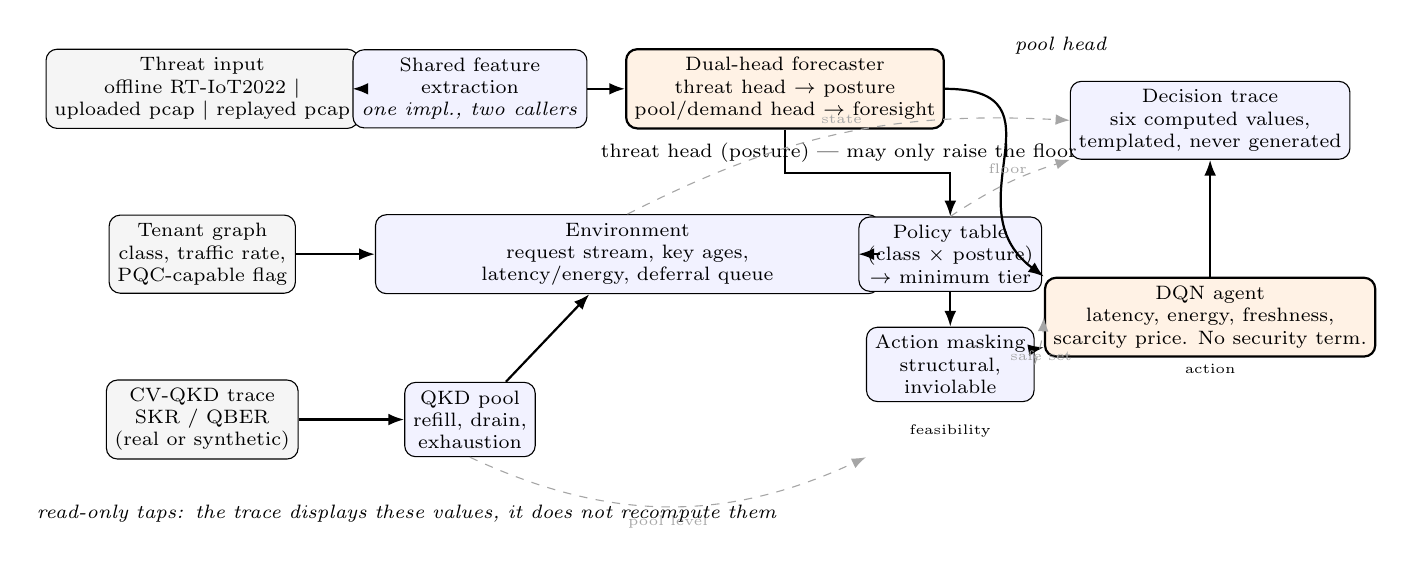
\begin{tikzpicture}[
  font=\scriptsize,
  box/.style={draw, rounded corners, align=center, minimum height=0.85cm, inner sep=3pt, fill=blue!5},
  input/.style={draw, rounded corners, align=center, minimum height=0.85cm, inner sep=3pt, fill=gray!8},
  agentbox/.style={draw, rounded corners, align=center, minimum height=1cm, inner sep=3pt, fill=orange!10, thick},
  tap/.style={draw, dashed, -{Latex[length=1.8mm]}, gray!70},
  flow/.style={-{Latex[length=2mm]}, thick}
]
\node[input] (threat) at (0,0) {Threat input\\ offline RT-IoT2022 $\vert$\\ uploaded pcap $\vert$ replayed pcap};
\node[box] (feat) at (3.4,0) {Shared feature\\ extraction\\ \emph{one impl., two callers}};
\node[agentbox] (forecaster) at (7.4,0) {Dual-head forecaster\\ threat head $\to$ posture\\ pool/demand head $\to$ foresight};

\node[input] (graph) at (0,-2.1) {Tenant graph\\ class, traffic rate,\\ PQC-capable flag};
\node[input] (cvqkd) at (0,-4.2) {CV-QKD trace\\ SKR / QBER\\ (real or synthetic)};
\node[box] (pool) at (3.4,-4.2) {QKD pool\\ refill, drain,\\ exhaustion};

\node[box, minimum width=6.4cm] (env) at (5.4,-2.1) {Environment\\ request stream, key ages,\\ latency/energy, deferral queue};

\node[box] (policy) at (9.5,-2.1) {Policy table\\ (class $\times$ posture)\\ $\to$ minimum tier};
\node[box] (mask) at (9.5,-3.5) {Action masking\\ structural,\\ inviolable};
\node[agentbox] (dqn) at (12.8,-2.9) {DQN agent\\ latency, energy, freshness,\\ scarcity price. No security term.};
\node[box] (trace) at (12.8,-0.4) {Decision trace\\ six computed values,\\ templated, never generated};

\draw[flow] (threat) -- (feat);
\draw[flow] (feat) -- (forecaster);
\draw[flow] (graph) -- (env);
\draw[flow] (cvqkd) -- (pool);
\draw[flow] (pool) -- (env);
\draw[flow] (forecaster.south) -- ++(0,-0.55) -| node[pos=0.02,above,xshift=6mm]{threat head (posture) --- may only raise the floor} (policy.north);
\draw[flow] (forecaster.east) .. controls +(1.6,0) and +(-1.2,0.9) .. (dqn.north west);
\node[align=center, font=\scriptsize\itshape] at (10.9,0.55) {pool head};
\draw[flow] (env.east) -- (policy.west);
\draw[flow] (policy) -- (mask);
\draw[flow] (mask) -- (dqn);
\draw[flow] (dqn) -- (trace);
\draw[tap] (env.north) to[bend left=15] node[above,font=\tiny]{state} (trace.west);
\draw[tap] (policy.north) to[bend left=8] node[above,font=\tiny]{floor} (trace.south west);
\draw[tap] (mask.east) to[bend right=8] node[below,font=\tiny]{safe set} (dqn.west);
\draw[tap] (pool.south) to[bend right=25] node[below,font=\tiny]{pool level} (mask.west |- pool.south);

\node[font=\tiny] at (9.5,-4.35) {feasibility};
\node[font=\tiny] at (12.8,-3.55) {action};

\node[font=\scriptsize\itshape, align=left, text width=17cm] at (6.4,-5.4)
 {read-only taps: the trace displays these values, it does not recompute them};
\end{tikzpicture}
\caption{SmartKeyNet architecture. The threat signal reaches the agent only through the policy table and the mask, never through the reward. Changing the input mode changes nothing downstream of the shared feature-extraction step, which is what makes the replayed-capture mode behaviorally equivalent to a live interface instead of a second, more forgiving pipeline.}
\label{fig:architecture}
\end{figure*}

\subsection{Pool dynamics}

The pool holds $B_t$ bits at step $t$ and refills from a secret-key-rate trace. Writing $R_t$ for the instantaneous secret-key rate the
trace delivers, $B_{\max}$ for pool capacity, and $D_t$ for the requests
served with hybrid material at step $t$ with per-request draw $b_i$,
\begin{equation}
B_{t+1} = \min\!\left( B_{\max},\; B_t + R_t \Delta t - \sum_{i \in D_t} b_i \right).
\label{eq:pool}
\end{equation}
$R_t$ falls as the quantum bit error rate rises, so a degradation
scenario is expressed entirely by supplying a trace in which
QBER climbs and $R_t$ collapses. We do not model the QKD
physical layer: the trace is the interface, and the pool is the
abstraction the decision layer sees, matching the ETSI view
of a key store behind a delivery API~\cite{ref6}.

\subsection{Threat estimation and the dual-head forecaster}

Network telemetry is windowed and reduced to flow-level
features by one extraction function with two callers: an offline
path consuming labeled intrusion data for training, and an
inference path consuming packets from a capture file. That
single implementation is what makes the three input modes of
Fig.~\ref{fig:architecture} interchangeable.

The forecaster is an LSTM~\cite{ref21} with two heads. The threat
head emits a scalar score $s_t \in [0,1]$ and a distribution $p_t$
over three postures $\mathcal{P} = \{\text{calm}, \text{elevated}, \text{high}\}$, resolved by
$\hat{p}_t = \arg\max p_t$. The pool-and-demand head projects the pool
level and the volume of floor-mandatory hybrid demand $H$
steps ahead. Only the second head reaches the agent's state;
the first reaches the policy table. That split is the mechanism
behind the anticipation claim: a threshold policy responds to
the pool level it can see, whereas foresight features let the
agent respond to the level it expects and conserve ahead of
a scarcity event. Whether that difference matters is what the
ablation in Section~\ref{sec:scenarios} measures.

The forecaster is trained offline and frozen; no gradient from
the DQN loss reaches it. Were it trainable end to end against
the agent's return, the agent would gain an indirect incentive
to influence its own constraint, and the separation this paper
is about would quietly stop holding. That is a design rule, not
an optimization detail.

\subsection{Policy floors and action masking}

Let $\varphi : \mathcal{C} \times \mathcal{P} \to T$ map a sensitivity class and a posture
to a minimum tier; Table~\ref{tab:floor} gives its structure. The table is
monotone in posture by construction:
\begin{equation}
p \preceq p' \implies \varphi(c,p) \preceq \varphi(c,p') \quad \forall c \in \mathcal{C}.
\label{eq:monotone}
\end{equation}
Equation~(\ref{eq:monotone}) is the formal content of ``the threat signal may
only raise floors,'' and a unit test checks it across the whole
table; we do not assume it.

\begin{table}[htbp]
\caption{Structure of the floor table $\varphi(c,p)$. Cells are calibrated against \cite{ref2}, \cite{ref3}, \cite{ref20}: configuration, not results}
\label{tab:floor}
\centering
\begin{tabular}{@{}L{2.6cm}ccc@{}}
\toprule
Sensitivity class $c$ & calm & elevated & high \\
\midrule
Public / telemetry & T0 & T1 & T1 \\
Internal & T1 & T1 & T2 \\
Confidential & T1 & T2 & T2 \\
Long-lived regulated & T2 & T2 & T3 \\
\bottomrule
\end{tabular}
\end{table}

Let $F_t$ hold the actions physically feasible at step $t$: hybrid
needs $B_t \geq b$, \texttt{REUSE} needs an existing key inside its age
cap, \texttt{REKEY\_NOW} needs an existing key. The safe action set
is
\begin{equation}
\mathcal{A}^{\text{safe}}_t = \{\, a \in \mathcal{A} : \tau(a) \succeq \varphi(c_t, \hat{p}_t) \,\} \cap F_t.
\label{eq:safeset}
\end{equation}
Fig.~\ref{fig:masking} works a single request through~(\ref{eq:safeset}). The environment
computes~(\ref{eq:safeset}) and hands the agent only $\mathcal{A}^{\text{safe}}_t$. Actions outside
it are not penalized, not discouraged, and not sampled during
exploration; they are absent. One consequence deserves stating
precisely, because it is the paper's central claim. Define the
below-floor service rate of a policy $\pi$ over $N$ decisions against
the true posture $p^{\star}_t$ rather than the estimated one:
\begin{equation}
V(\pi) = \frac{1}{N} \sum_{t=1}^{N} \mathbb{1}\!\left[\, \tau(a_t) \prec \varphi(c_t, p^{\star}_t) \,\right], \quad a_t \sim \pi.
\label{eq:belowfloor}
\end{equation}
For any policy restricted to~(\ref{eq:safeset}) and any estimate $\hat{p}_t \succeq p^{\star}_t$,
every selectable action satisfies $\tau(a_t) \succeq \varphi(c_t, \hat{p}_t) \succeq \varphi(c_t, p^{\star}_t)$
by~(\ref{eq:monotone}), so $V(\pi) = 0$ identically. The guarantee needs neither
training, convergence, nor an accurate estimator --- only one
that does not under-estimate. Driving $\hat{p}_t$ upward leaves the
bound intact; driving it downward is the case Section~\ref{sec:steering} measures.

\begin{figure}[t]
\centering
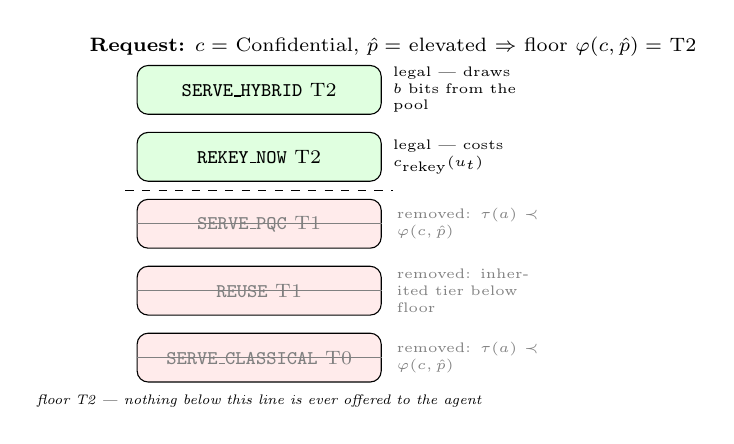
\begin{tikzpicture}[
  font=\scriptsize,
  legal/.style={draw, rounded corners, fill=green!12, minimum width=3.1cm, minimum height=0.62cm, align=left, inner sep=3pt},
  illegal/.style={draw, rounded corners, fill=red!8, minimum width=3.1cm, minimum height=0.62cm, align=left, inner sep=3pt, text=gray},
  every node/.style={font=\scriptsize}
]
\node[align=center] at (1.7,0.55) {\textbf{Request:} $c=$ Confidential, $\hat{p}=$ elevated $\Rightarrow$ floor $\varphi(c,\hat{p})=$ T2};

\node[legal] (hybrid) at (0,0) {\texttt{SERVE\_HYBRID} \hfill T2};
\node[legal] (rekey) at (0,-0.85) {\texttt{REKEY\_NOW} \hfill T2};
\node[illegal] (pqc) at (0,-1.7) {\texttt{SERVE\_PQC} \hfill T1};
\node[illegal] (reuse) at (0,-2.55) {\texttt{REUSE} \hfill T1};
\node[illegal] (classical) at (0,-3.4) {\texttt{SERVE\_CLASSICAL} \hfill T0};
\draw[gray] (pqc.west) -- (pqc.east);
\draw[gray] (reuse.west) -- (reuse.east);
\draw[gray] (classical.west) -- (classical.east);

\draw[dashed] (-1.7,-1.28) -- (1.7,-1.28);
\node[align=left, text width=1.7cm, font=\tiny] at (2.55,0) {legal --- draws $b$ bits from the pool};
\node[align=left, text width=1.7cm, font=\tiny] at (2.55,-0.85) {legal --- costs $c_{\text{rekey}}(u_t)$};
\node[align=left, text width=1.9cm, font=\tiny, text=gray] at (2.7,-1.7) {removed: $\tau(a)\prec\varphi(c,\hat{p})$};
\node[align=left, text width=1.9cm, font=\tiny, text=gray] at (2.7,-2.55) {removed: inherited tier below floor};
\node[align=left, text width=1.9cm, font=\tiny, text=gray] at (2.7,-3.4) {removed: $\tau(a)\prec\varphi(c,\hat{p})$};
\node[font=\tiny\itshape] at (0,-3.95) {floor T2 --- nothing below this line is ever offered to the agent};
\end{tikzpicture}
\caption{One request through~(\ref{eq:safeset}). The floor is a table lookup, the strike-outs
are the three legality rules \texttt{compute\_mask()} implements, and the learned
policy only ever ranks what survives. Actions below the floor are absent from
the action set, not penalized within it. $\mathcal{A}^{\text{safe}}_t = \{\texttt{SERVE\_HYBRID}, \texttt{REKEY\_NOW}\}$; the agent takes $\arg\max_a Q_\theta(s_t,a)$ over those two. If $B_t < b$ the first also leaves $F_t$, the set empties, and the request is deferred rather than downgraded.}
\label{fig:masking}
\end{figure}

\begin{algorithm}[t]
\caption{Per-request decision}
\label{alg:decision}
\begin{algorithmic}[1]
\Require request $(m, v, c_t)$, state $s_t$, pool $B_t$, posture $\hat{p}_t$
\State $f \gets \varphi(c_t, \hat{p}_t)$ \Comment{table lookup, no judgment}
\State $\mathcal{A}^{\text{safe}}_t \gets \{ a : \tau(a) \succeq f \} \cap F_t$
\If{$\mathcal{A}^{\text{safe}}_t = \emptyset$}
    \State defer request; log regret event \Comment{never downgrade}
    \State \Return
\EndIf
\State $a_t \gets \arg\max_{a \in \mathcal{A}^{\text{safe}}_t} Q_\theta(s_t, a)$
\State record $(s^{\text{thr}}_t, p_t, f, \mathcal{A}^{\text{safe}}_t, \text{costs}, a_t)$ for the trace
\State apply $a_t$; update $B_{t+1}$ by~(\ref{eq:pool})
\end{algorithmic}
\end{algorithm}

\subsection{Reward design without a security term}

Inside the safe set the agent optimizes an operational
objective only:
\begin{align}
r_t = {} & -w_{\text{lat}} \ell_t - w_{\text{ene}} e_t + w_{\text{fr}} \phi_t \nonumber \\
         & - w_{\text{qkd}} \beta_t - R_{\text{starve}} d_t - c_{\text{rekey}}(u_t)\, \mathbb{1}[\text{rekey}],
\label{eq:reward}
\end{align}
where $\ell_t$ is served latency, $e_t$ energy, $\phi_t$ key freshness, $\beta_t$
pool bits consumed this step, $d_t$ the number of steps a floor-mandatory request sits deferred, and $u_t \in [0,1]$ instantaneous
load. Rekey cost grows with load as $c_{\text{rekey}}(u) = c_0(1 + \beta u)$,
so forced refreshes are cheap when the service is idle and
expensive during a burst. We set $R_{\text{starve}}$ roughly an order of
magnitude above $w_{\text{lat}}$, making deferral the most expensive
routine outcome in~(\ref{eq:reward}) without ever making a downgrade
available as an alternative. Latency and energy coefficients are
taken from published primitive benchmarks~\cite{ref22}, \cite{ref23} and not
fitted. We would rather state the limit of that claim than lean on
it: those benchmarks were measured on general-purpose and
embedded platforms, not on a KMS host, so the coefficients
are grounded in measurement without being calibrated to our
setting.

\begin{figure}[t]
\centering
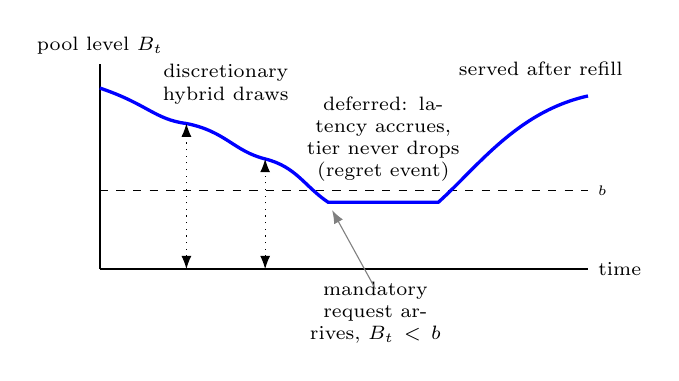
\begin{tikzpicture}[font=\scriptsize, >=Latex]
\draw[thick] (0,0) -- (6.2,0) node[right] {time};
\draw[thick] (0,0) -- (0,2.6) node[above] {pool level $B_t$};
\draw[dashed] (0,1.0) -- (6.2,1.0) node[right, font=\tiny] {$b$};

\draw[very thick, blue] (0,2.3)
 .. controls (0.6,2.1) and (0.7,1.9) .. (1.1,1.85)
 .. controls (1.6,1.75) and (1.7,1.5) .. (2.1,1.4)
 .. controls (2.5,1.3) and (2.6,1.05) .. (2.9,0.85)
 -- (4.3,0.85)
 .. controls (4.8,1.3) and (5.3,2.0) .. (6.2,2.2);

\draw[<->, dotted] (1.1,0) -- (1.1,1.85);
\draw[<->, dotted] (2.1,0) -- (2.1,1.4);

\node[align=center, text width=2.1cm] at (1.6,2.35) {discretionary hybrid draws};
\node[align=center, text width=2.3cm] at (3.5,-0.55) {mandatory request arrives, $B_t < b$};
\draw[->, gray] (3.5,-0.25) -- (2.95,0.75);

\node[align=center, text width=2.6cm] at (3.6,1.65) {deferred: latency accrues,\\ tier never drops (regret event)};

\node[align=center, text width=2.2cm] at (5.6,2.55) {served after refill};
\end{tikzpicture}
\caption{Why the decisions are coupled, drawn schematically. Discretionary
hybrid draws early in the window are the reason a later floor-mandatory
request finds $B_t < b$ and waits. Hard rule: the request is queued, never
served below its floor. Axes are deliberately unnumbered --- this illustrates
the mechanism defined by~(\ref{eq:pool}) and Algorithm~\ref{alg:decision}, and is not simulation output.}
\label{fig:coupling}
\end{figure}

No term in~(\ref{eq:reward}) is proportional to a threat score, a tier, or
a posture, and we do not relax this even temporarily during
training: a security term added ``to help early convergence''
reintroduces exactly the gradient an adversary shapes. The
agent is a double DQN~\cite{ref24} whose bootstrap target maximizes
over the safe set at the successor state,
\begin{equation}
y_t = r_t + \gamma \max_{a' \in \mathcal{A}^{\text{safe}}_{t+1}} Q_{\theta^-}(s_{t+1}, a').
\label{eq:target}
\end{equation}
Masking the target as well as the behavior policy matters:
if~(\ref{eq:target}) maximized over the full action set, the value function
would expect returns from actions it can never take, and the
bias would surface as over-optimistic values in exactly the
high-posture states where the mask is tightest.

\subsection{Deferral and regret accounting}

Fig.~\ref{fig:coupling} draws the coupling that makes this a budgeting
problem rather than a sequence of independent choices. Pool
exhaustion makes~(\ref{eq:safeset}) empty, which Algorithm~\ref{alg:decision} resolves by
queuing the request: it waits, accrues latency, and is served
when refill permits. We log the onset of each wait as a regret
event, since it marks a moment when earlier discretionary
spending removed a later mandatory option. Regret and exhaustion counts measure misbudgeting in one direction; rekey
ratio and p99 latency measure over-conservation in the other,
and reporting both matters because a policy that hoards scores
perfectly on the first pair while being useless. Exhaustion is
an availability failure the agent pays for, never a security
failure, and that framing is what lets the guarantee after~(\ref{eq:belowfloor})
be unconditional.

\subsection{Decision traces}

Fig.~\ref{fig:trace} shows the six values Algorithm~\ref{alg:decision} records per decision. Each is a real intermediate result read off the environment, the policy table, or the agent at decision time, and the
interface renders those and nothing else. Text is produced by
substituting the values into fixed templates, so the sentence
a reviewer reads is a rendering of the computation, not a
description of it.

The interface degrades honestly where a naive explanation
would overclaim: with one legal action left, step 5 reports
that no cost comparison took place instead of showing a one-row table as though a tradeoff had been evaluated, and when
the learned preference broke a tie among comparable options,
step 6 says so.

\begin{figure}[t]
\centering
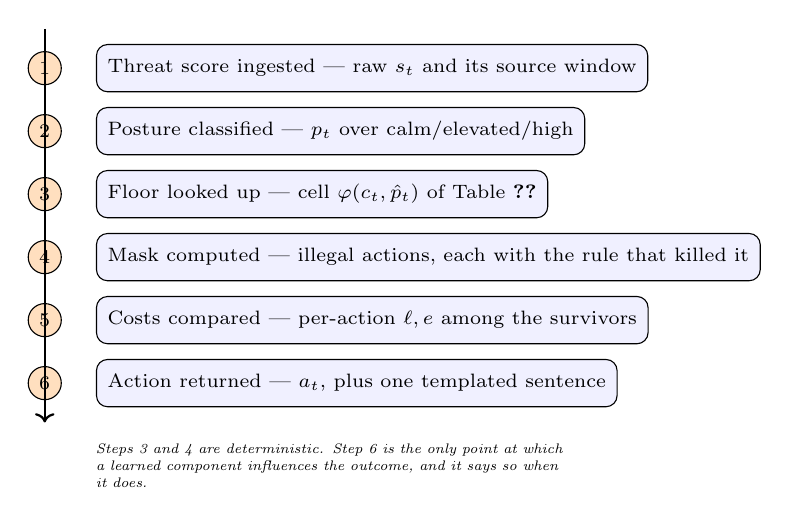
\begin{tikzpicture}[
  font=\scriptsize,
  stepbox/.style={draw, rounded corners, fill=blue!6, anchor=west, minimum width=4.7cm, minimum height=0.6cm, align=left, inner sep=4pt},
  numcirc/.style={draw, circle, fill=orange!25, minimum size=0.42cm, inner sep=0pt}
]
\foreach \i/\txt/\y in {
  1/{Threat score ingested --- raw $s_t$ and its source window}/0,
  2/{Posture classified --- $p_t$ over calm/elevated/high}/-0.8,
  3/{Floor looked up --- cell $\varphi(c_t,\hat p_t)$ of Table~\ref{tab:floor}}/-1.6,
  4/{Mask computed --- illegal actions, each with the rule that killed it}/-2.4,
  5/{Costs compared --- per-action $\ell,e$ among the survivors}/-3.2,
  6/{Action returned --- $a_t$, plus one templated sentence}/-4.0
}{
  \node[stepbox] (b\i) at (-1.3,\y) {\txt};
  \node[numcirc] at (-1.95,\y) {\i};
}
\draw[->, thick] (-1.95,0.5) -- (-1.95,-4.5);
\node[align=left, text width=6.0cm, font=\tiny\itshape] at (1.7,-5.05)
 {Steps 3 and 4 are deterministic. Step 6 is the only point at which a learned component influences the outcome, and it says so when it does.};
\end{tikzpicture}
\caption{The six values recorded per decision by Algorithm~\ref{alg:decision}. Nothing shown
is reconstructed after the fact and no sentence is generated: text comes from
substitution into fixed templates.}
\label{fig:trace}
\end{figure}

\section{Experimental Setup}
\label{sec:impl}

\subsection{Data provenance}

External data enters at exactly three points (Table~\ref{tab:provenance}).
Everything else (pool arithmetic, key sizes, request arrival,
the floor-ratchet schedule) is simulator configuration, and we
prefer to say so plainly; calling configuration a dataset would
be dressing it up.

\begin{table*}[t]
\caption{Data provenance. Only the first three rows are external data}
\label{tab:provenance}
\centering
\begin{tabular}{@{}L{3.6cm}L{6.5cm}L{6.5cm}@{}}
\toprule
Component & Source & Role \\
\midrule
Forecaster, training & RT-IoT2022 labeled flows~\cite{ref25} & Offline training of both heads \\
Forecaster, inference & .pcap via the same extraction function & Alternate input path; identical feature shape is unit-tested \\
Pool refill & Published field-trial SKR/QBER data~\cite{ref4}, \cite{ref26}, or a documented synthetic process & Drives $R_t$ in~(\ref{eq:pool}); the synthetic process is what runs today \\
Latency, energy & liboqs~\cite{ref22}, pqm4~\cite{ref23} & Coefficients in~(\ref{eq:reward}); benchmarked, not fitted \\
Draw and key sizes; tenant graph; S6 floor schedule & ETSI GS QKD 014~\cite{ref6}; seeded generator; config file & Simulator arithmetic; graph and schedule are exogenous and invisible to the agent \\
\bottomrule
\end{tabular}
\end{table*}

One negative constraint governs the reward-shaped baseline:
its logs calibrate it and never train the masked agent, since that
would be imitation learning of the precise policy the attack
is meant to break. We also screen every input file for label
degeneracy: one in which a single label covers nearly the
whole set is discarded, not sampled around. We found such
a file during preparation, and catching it after training would
have cost more than the screen does.

\begin{figure}[t]
\centering
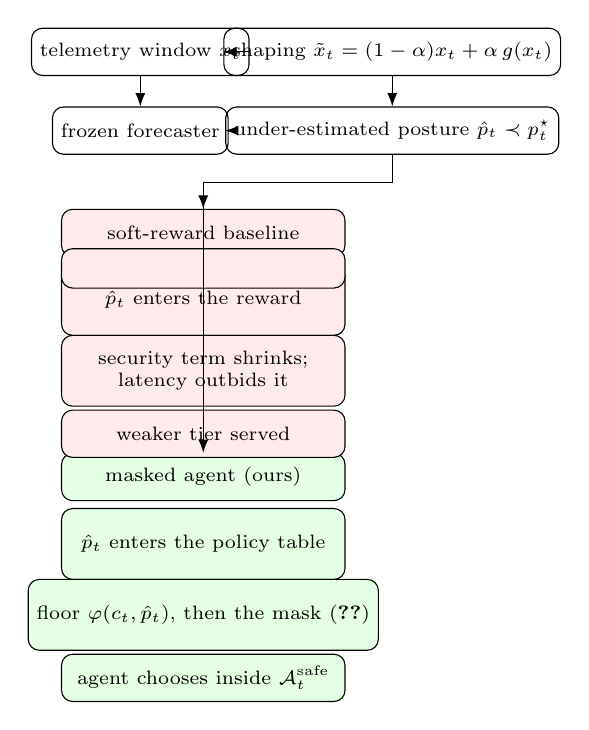
\begin{tikzpicture}[
  font=\scriptsize,
  block/.style={draw, rounded corners, align=center, minimum height=0.6cm, inner sep=3pt},
  softbox/.style={draw, rounded corners, align=center, minimum height=0.6cm, inner sep=3pt, fill=red!8},
  maskbox/.style={draw, rounded corners, align=center, minimum height=0.6cm, inner sep=3pt, fill=green!10},
  ->,>=Latex
]
\node[block] (window) at (0,0) {telemetry window $x_t$};
\node[block] (shape) at (3.2,0) {shaping $\tilde x_t = (1-\alpha)x_t + \alpha\, g(x_t)$};
\node[block] (froz) at (0,-1) {frozen forecaster};
\node[block] (under) at (3.2,-1) {under-estimated posture $\hat p_t \prec p^\star_t$};

\node[softbox, minimum width=3.6cm] (soft) at (0.8,-2.3) {soft-reward baseline};
\node[maskbox, minimum width=3.6cm] (masked) at (0.8,-5.4) {masked agent (ours)};

\node[softbox, minimum width=3.6cm, minimum height=0.9cm] (s1) at (0.8,-3.15) {$\hat p_t$ enters the reward};
\node[softbox, minimum width=3.6cm, minimum height=0.9cm] (s2) at (0.8,-4.05) {security term shrinks;\\ latency outbids it};
\node[softbox, minimum width=3.6cm, minimum height=0.6cm] (s3) at (0.8,-4.85) {weaker tier served};
\node[softbox, minimum width=3.6cm, minimum height=0.5cm, font=\bfseries\scriptsize] (s4) at (0.8,-2.75) {};

\node[maskbox, minimum width=3.6cm, minimum height=0.9cm] (m1) at (0.8,-6.25) {$\hat p_t$ enters the policy table};
\node[maskbox, minimum width=3.6cm, minimum height=0.9cm] (m2) at (0.8,-7.15) {floor $\varphi(c_t,\hat p_t)$, then the mask~(\ref{eq:safeset})};
\node[maskbox, minimum width=3.6cm, minimum height=0.6cm] (m3) at (0.8,-7.95) {agent chooses inside $\mathcal{A}^{\text{safe}}_t$};

\draw (window) -- (shape);
\draw (froz) -- (under);
\draw (window) -- (froz);
\draw (shape) -- (under);
\draw (under.south) -- ++(0,-0.35) -| (soft.north);
\draw (under.south) -- ++(0,-0.35) -| (masked.north);
\end{tikzpicture}
\caption{Where an adversarially shaped threat signal lands in each design.
The perturbation is identical; only its destination differs. A reward term is a
preference an attacker can bid down, while a floor is a constraint the same
attacker can only tighten. The right-hand outcome follows from~(\ref{eq:monotone}) and~(\ref{eq:safeset}), not from training.}
\label{fig:steering}
\end{figure}

\subsection{Scenarios and baselines}
\label{sec:scenarios}

Table~\ref{tab:scenarios} lists the grid. S1--S4 are training environments;
S5 and S6 are held out. The separation matters most for S6,
since an agent trained on the migration schedule would learn
its timing instead of a general conservation habit.

\begin{table}[htbp]
\caption{Scenario grid}
\label{tab:scenarios}
\centering
\begin{tabular}{@{}lL{4.6cm}l@{}}
\toprule
ID & What changes & Split \\
\midrule
S1 & Steady mixed traffic & Train \\
S2 & Threat elevates; floors ratchet up & Train \\
S3 & QBER rises, SKR falls, refill collapses & Train \\
S4 & One low-sensitivity tenant floods the API & Train \\
S5 & Adversarially shaped threat trace & Eval \\
S6 & Scripted floor-ratchet migration schedule & Held out \\
E-A & Foresight source varied: off / EWMA / LSTM & Eval \\
\bottomrule
\end{tabular}
\end{table}

Four non-RL baselines are mandatory: always-PQC, always-hybrid, a static threshold on pool level grid-searched per
scenario, and uniform random selection over the safe set. The
third is the one that matters: if a tuned threshold matches
the masked DQN, the premise of this work is weak, and we
have committed in advance to reporting that and examining the
environment before defending the method. A fifth baseline, the
reward-shaped agent, gives the attack a target.

\subsection{Steering attack protocol}
\label{sec:steering}

The attack shapes the telemetry reaching the forecaster
so the estimated posture is biased downward. Parameterizing
attack strength by $\alpha \in [0,1]$, the observed feature window
becomes
\begin{equation}
\tilde{x}_t = (1-\alpha)\, x_t + \alpha\, g(x_t),
\label{eq:steering}
\end{equation}
where $g$ maps a window toward the benign region of the
learned feature space. Fig.~\ref{fig:steering} shows where that shaped signal
lands in each design.

We sweep $\alpha$ in eleven steps and report $V(\pi)$ from~(\ref{eq:belowfloor})
against the true posture the simulator knows and the agent
does not, for both policies, with served-tier histograms at three
checkpoints. The prediction is asymmetric and we state it
before running: the baseline's curve should rise with $\alpha$, its
payoff for a stronger tier shrinking as perceived threat falls,
while the masked agent's stays flat at zero for the structural
reason after~(\ref{eq:belowfloor}). A nonzero value there would indicate a bug
in the mask, not a limit of the argument.

\subsection{Metrics and implementation status}

We report p99 latency, pool-exhaustion count, regret events,
forced-rekey ratio, and below-floor service rate per policy per
scenario, over ten seeds, as medians with interquartile ranges
instead of means, since the exhaustion distribution is skewed
by construction.

The rest of the paper depends on stating the following
plainly. Implemented and tested: the pool simulator, the deferral queue and regret accounting, the masking logic and
floor lookup, the environment wiring these together with~(\ref{eq:reward}),
the masked DQN, the reward-shaped baseline, the four non-RL baselines, and the scenario comparison runner. This spine
runs end to end on S1 and S3, and Section~\ref{sec:results} reports S3.
Partial: the forecaster has only a non-learned exponentially-weighted-moving-average fallback over a placeholder signal,
so the dual-head model of Section~III-D does not exist yet, and
the S3 numbers therefore exercise the masking and budgeting
machinery under a stub threat signal; the request stream is
synthetic and not yet a graph sample; scenario dispatch for
S2, S4 and S6 is configured but not acted on. Not started:
the trace generator of~(\ref{eq:steering}) and the dose-response sweep, and
the operator interface, which exists only as a hand-authored
mockup with fabricated values that we neither reproduce nor
cite.

\section{Results and Discussion}
\label{sec:results}

\subsection{What holds without a run}

One result does not require a run. The bound $V(\pi) = 0$
after~(\ref{eq:belowfloor}) is a property of~(\ref{eq:safeset}) and~(\ref{eq:monotone}) together, so it holds
for every representable policy at every point in training under
every threat trace. We verify it by assertion in the environment,
not by measurement: the assertion fires on the first violation,
not after enough of them to move an average. Everything else
below is measured, and carries the caveats it has earned.

\subsection{S3: budgeting under a collapsing key rate}

Table~\ref{tab:results} gives the S3 grid: QBER climbs, the secret-key rate
falls, and pool refill stops covering demand. Six policies, ten
seeds, medians.

\begin{table*}[t]
\caption{Scenario S3 (QKD degradation), ten seeds, median. Exhaustion and regret are event counts; below-floor is the count of decisions served under the floor, the numerator of~(\ref{eq:belowfloor})}
\label{tab:results}
\centering
\begin{tabular}{@{}lccccc@{}}
\toprule
Policy & p99 lat.\footnotemark[1] & Exhaust. & Regret & Rekey \% & Below-floor \\
\midrule
Masked DQN (ours) & 150.0 & 0.0 & 0.0 & 12.1 & 0 \\
Soft-reward DQN & 120.0 & 19.5 & 19.5 & 9.5 & 27,301 \\
Static threshold & 150.0 & 42.0 & 42.0 & 6.9 & 0 \\
Always-hybrid & 150.0 & 676.0 & 676.0 & 93.5 & 0 \\
Always-PQC & 150.0 & 531.0 & 531.0 & 95.5 & 0 \\
Random (safe set) & 150.0 & 510.5 & 510.5 & 66.0 & 0 \\
\bottomrule
\end{tabular}

\footnotetext[1]{Simulator time units. See Section~\ref{sec:instrumentation} on the saturation visible in this column.}
\end{table*}

The separation the paper argues for shows up in the last column. The masked agent serves nothing below its floor, which
is what~(\ref{eq:safeset}) guarantees. The reward-shaped agent, trained on the
same environment with the same forecaster and differing only
in where the threat signal enters, serves 27,301 decisions below
floor. Being precise about what that does and does not show:
it is not the steering attack, since no adversary was present. It
shows that a security term weighted against latency and energy
is traded away under ordinary scarcity, before anyone tries to
manipulate it. The attack of~(\ref{eq:steering}) makes that trade worse on
purpose, and it remains unrun.

What the reward-shaped agent buys with those decisions
sits two columns over: the lowest p99 in the grid and a rekey
ratio below the masked agent's. It is the only policy that beats
the masked agent on a performance metric, and it does so by
serving weaker keys. That is the finding, and burying it would
be the wrong instinct: on the metrics an operator watches, the
unsafe design looks better.

\subsection{The threshold comparison, which we committed to reporting either way}

Section~\ref{sec:scenarios} committed us in advance to reporting a tie
with the tuned threshold if one occurred. There is no tie, and
no clean win either. The threshold matches the masked agent
on p99 and beats it on rekey churn, 6.9\% against 12.1\%, but
reaches 42 pool-exhaustion events where the masked agent
reaches zero. The agent is buying availability with churn,
rekeying roughly twice as often on cheaper tiers to hold pool
material in reserve for requests whose floor will demand it.
Whether that is worth 5.2 points of rekey ratio is an operator's
judgement, but the direction is the one the design intends.

The static baselines behave as the scarcity argument predicts. Always-hybrid drains the pool and exhausts 676 times.
Always-PQC is the more interesting case: it never prefers
pool material, yet still exhausts 531 times, because masking
forces it to hybrid whenever a floor demands T2 and it has
done nothing beforehand to conserve. Non-anticipation, not
appetite, is what exhausts it.

\subsection{Failure modes: one materialized, one did not}

Section~\ref{sec:scenarios} named over-conservation as a risk, on the
grounds that a large $R_{\text{starve}}$ pushes toward hoarding. It materialized: the masked agent's rekey ratio is 1.8 times the
threshold's, and its zero-exhaustion record is partly bought
that way. We flagged this in advance and report both columns
for exactly this reason, since a table carrying only regret and
exhaustion would have shown a perfect score and hidden the
cost. The threshold tie did not materialize, so the premise
survives its own disqualification rule. The third named risk,
the attack's sensitivity to the baseline's security weight, cannot
be assessed until the sweep runs.

\subsection{Instrumentation issues we have not resolved}
\label{sec:instrumentation}

Two features of Table~\ref{tab:results} we do not yet trust, and flagging
them is better than interpreting them.

Five of six policies report a p99 latency of exactly 150.0.
Policies whose exhaustion counts differ by two orders of
magnitude should not agree to one decimal place on a tail
statistic. The likely explanation is a ceiling in the latency
model or the deferral timeout, in which case the column
reports saturation and not behavior, and only the reward-shaped agent's 120.0 reflects anything. We draw no conclusion
from it until the cap is located.

Exhaustion and regret coincide exactly in all six rows,
though Section~III-G treats them as distinct: one counts
moments the pool cannot cover a draw, the other the onset of
a deferral caused by earlier discretionary spending. An exact
identity across six policies and ten seeds means either that
the counters are wired to the same event, or that every S3
exhaustion happens to produce exactly one deferral onset. We
have not established which, so for now the two columns should
be read as one measurement reported twice.

\subsection{Limitations}

The security argument is narrow. Masking guarantees that
no served key falls below the floor the table specifies; it says
nothing about whether the table is right, and a mis-specified
floor is a failure the mechanism cannot detect. The guarantee
also assumes the estimator does not under-estimate, which
(\ref{eq:steering}) is designed to violate; masking survives because under-estimation costs the masked system nothing, not because it
prevents under-estimation.

We measured this boundary directly. Sweeping attack strength $\alpha$
in eleven steps on S2, the masked agent's below-floor service rate
$V(\pi)$, averaged over 5 eval seeds, is $0.0000$ for $\alpha \le 0.4$,
stays near zero ($0.0016$--$0.0096$) for $\alpha = 0.5$--$0.8$, then
jumps to $0.3000$ at $\alpha \ge 0.9$. Tracing the mechanism directly
rules out a masking defect: the count of decisions delivered below the
floor the mask was actually shown is exactly zero at every seed and
every $\alpha$, so~(\ref{eq:safeset}) and~(\ref{eq:monotone}) hold
without exception throughout. What moves is the floor computation
upstream of the mask. At $\alpha=0.7$ a single seed's per-decision
trace shows two violating decisions immediately after the scripted
threat elevation begins; the ratchet catches the diluted but still
nonzero true signal within two decisions and locks the floor up for
the rest of the episode. At $\alpha \ge 0.9$ the same trace shows
violations persisting for the remainder of the episode: the shaped
signal never carries enough of the true elevation through for the
estimator to cross the posture threshold at any point, so the ratchet
is never given a genuine reading to lock onto. We tested the natural
mitigation this suggests --- shaping the signal only from the scripted
elevation onward and leaving every earlier tick honest --- and it does
not restore the guarantee: masked $V(\pi)$ still reaches $0.3000$ at
$\alpha \ge 0.9$, nearly identical to the unrestricted sweep. An honest
reading before the attack begins is therefore not by itself a
mitigation; what the ratchet needs is an honest reading during the
elevation itself, and a sufficiently strong attack denies exactly
that, regardless of what came before it. The guarantee, stated
precisely, is narrower than it first appears: masking cannot be talked
out of a floor it has already locked in, but it cannot lock in a floor
from a reading the attack suppressed at the one moment that reading
mattered.

The soft-reward baseline's own reward does not read the estimated
threat probability or posture directly: its security term is a fixed
three-value lookup keyed only on the tier actually delivered, with no
continuous threat-weighted component for the attack to shrink. The one
exception is narrow and discrete: \texttt{REKEY\_NOW}'s delivered tier
resolves to the maximum of the existing tier and the current floor,
the same one-way-ratcheted $\varphi(c_t, \hat{p}_t)$ the masked
agent's own mask reads, so an attack that pulls this upstream quantity
down can lower what a \texttt{REKEY\_NOW} decision delivers without
the agent's policy choosing differently. We verified this directly:
across every tier-establishing decision ($100$ total, \texttt{SERVE\_*}
or \texttt{REKEY\_NOW}) at $\alpha=0.9$ over 5 eval seeds, 16 decisions
had a true/attacked posture-bucket divergence. In none of the 16 did
the learned policy's chosen action change under a true-posture
substitution with every other state field held fixed --- the agent
picks \texttt{REKEY\_NOW} regardless. But in 6 of those 16, the tier
that same, unchanged decision delivered did change, because the
resolution formula reads the attacked floor directly. The curve's
flat-then-step shape follows the same discrete posture-bucket-crossing
mechanism established above for the masked agent: a finer-resolution
sweep pins the crossing to $\alpha = 0.80 \to 0.85$, where the
posture-bucket-mismatch rate jumps from $0.0224$ to $0.8112$ in exact
step with $V(\pi)$ rising from $0.2896$ to $0.3256$. Despite reward
functions built on opposite premises --- one with no security term at
all, one with a fixed tier-only term --- both agents' only real point
of leverage for this attack turns out to be the same shared upstream
quantity: the one-way-ratcheted floor computed by the attackable
forecaster. Neither agent's reward is what the attack actually
reaches; both are reached only through this one shared channel.

The numbers come from one scenario with a stub threat
signal, so they exercise budgeting and masking but not anticipation: the foresight features of Section~III-D are not yet real,
and the masked agent's margin over the threshold is a floor on
what a working forecaster would give, not a measurement of
it. The evaluation is simulated throughout, and the primitive
costs, while benchmarked, come from platforms unlike a
KMS host. QKD is modeled as a rate trace, so physical-layer
attacks are outside the model. Availability under a determined
adversary is weaker here than confidentiality: an attacker who
inflates the posture drives the system toward hybrid, drains
the pool, and induces deferrals. Trading confidentiality risk
for availability risk is the right direction in our view, but it is
a trade, and the exhaustion and rekey columns are where its
cost appears.

\section{Conclusion and Future Work}

We have described a decision layer for a multi-tenant KMS
in which a deep Q-network budgets scarce QKD pool material
across tenants while being structurally unable to serve a key
below its policy floor. Masking over a monotone floor table,
rather than a weighted reward term, separates what the agent
optimizes from what the operator requires, and the consequence is a per-decision guarantee that survives an adversary
shaping the threat estimator's input. The same structure makes
each decision auditable, because every value behind an action
is a lookup or a comparison that already exists.

S3 shows the separation holding under ordinary scarcity:
zero below-floor decisions against 27,301, bought with rekey
churn we report rather than hide. What remains, in order:
locate the latency ceiling and separate the exhaustion and
regret counters, so Table~\ref{tab:results} can be read at face value; train the
dual-head forecaster on RT-IoT2022 and retire the moving-average fallback; implement the trace generator of~(\ref{eq:steering}) and
run the dose-response sweep, which is the result the design
was built to produce; and enable scenario dispatch for S2, S4
and S6. Longer term, deriving the floor table from compliance
documents in a checkable way is harder than it first appears,
and extending the pool model to a multi-node QKD network
with relayed keys would change the problem qualitatively,
since pool material would then have a location as well as a
quantity.

\begin{thebibliography}{00}
\bibitem{ref1} M. Mosca, ``Cybersecurity in an era with quantum computers: Will we
be ready?,'' \emph{IEEE Security \& Privacy}, vol. 16, no. 5, pp. 38--41, 2018.

\bibitem{ref2} National Institute of Standards and Technology, ``Module-lattice-based
key-encapsulation mechanism standard,'' FIPS 203, Aug. 2024, doi:
10.6028/NIST.FIPS.203.

\bibitem{ref3} National Security Agency, ``Announcing the Commercial National Security Algorithm Suite 2.0,'' NSA Cybersecurity Advisory, Sep. 2022.

\bibitem{ref4} M. Sasaki et al., ``Field test of quantum key distribution in the Tokyo
QKD Network,'' \emph{Optics Express}, vol. 19, no. 11, p. 10387, 2011, doi:
10.1364/OE.19.010387.

\bibitem{ref5} M. Mehic et al., ``Quantum key distribution: A networking perspective,'' \emph{ACM Computing Surveys}, vol. 53, no. 5, pp. 1--41, 2020, doi:
10.1145/3402192.

\bibitem{ref6} ETSI, ``Quantum key distribution (QKD); protocol and data format of
REST-based key delivery API,'' ETSI GS QKD 014 V1.1.1, Feb. 2019.

\bibitem{ref7} A. Uprety and D. B. Rawat, ``Reinforcement learning for IoT security:
A comprehensive survey,'' \emph{IEEE Internet of Things Journal}, vol. 8, no.
11, pp. 8693--8706, 2021, doi: 10.1109/JIOT.2020.3040957.

\bibitem{ref8} T. T. Nguyen and V. J. Reddi, ``Deep reinforcement learning for cyber
security,'' \emph{IEEE Transactions on Neural Networks and Learning Systems},
vol. 34, no. 8, pp. 3779--3795, Aug. 2023.

\bibitem{ref9} S. Huang, N. Papernot, I. Goodfellow, Y. Duan, and P. Abbeel, ``Adversarial attacks on neural network policies,'' in \emph{Proc. ICLR Workshop
Track}, 2017.

\bibitem{ref10} S. Huang and S. Ontan\'{o}n, ``A closer look at invalid action masking in
policy gradient algorithms,'' in \emph{Proc. 35th Int. FLAIRS Conf.}, 2022.

\bibitem{ref11} J. Garc\'{i}a and F. Fern\'{a}ndez, ``A comprehensive survey on safe reinforcement learning,'' \emph{Journal of Machine Learning Research}, vol. 16, no. 42,
pp. 1437--1480, 2015.

\bibitem{ref12} J. Achiam, D. Held, A. Tamar, and P. Abbeel, ``Constrained policy
optimization,'' in \emph{Proc. 34th Int. Conf. Machine Learning}, 2017, pp.
22--31.

\bibitem{ref13} V. Behzadan and A. Munir, ``Vulnerability of deep reinforcement learning to policy induction attacks,'' in \emph{Machine Learning and Data Mining
in Pattern Recognition}, 2017, pp. 262--275.

\bibitem{ref14} H.-K. Lo, M. Curty, and B. Qi, ``Measurement-device-independent
quantum key distribution,'' \emph{Physical Review Letters}, vol. 108, 130503,
2012, doi: 10.1103/PhysRevLett.108.130503.

\bibitem{ref15} S.-K. Liao et al., ``Satellite-to-ground quantum key distribution,'' \emph{Nature},
vol. 549, pp. 43--47, 2017, doi: 10.1038/nature23655.

\bibitem{ref16} A. Raj and V. Balachandran, ``A hybrid encryption framework combining
classical, post-quantum, and QKD methods,'' arXiv:2509.10551, Sep.
2025.

\bibitem{ref17} Y. Cao, Y. Zhao, J. Li, R. Lin, J. Zhang, and J. Chen, ``Multi-tenant
provisioning for quantum key distribution networks with heuristics and
reinforcement learning: A comparative study,'' \emph{IEEE Transactions on
Network and Service Management}, vol. 17, no. 2, pp. 946--957, 2020,
doi: 10.1109/TNSM.2020.2964003.

\bibitem{ref18} H. Krawczyk and P. Eronen, ``HMAC-based extract-and-expand key
derivation function (HKDF),'' IETF RFC 5869, May 2010.

\bibitem{ref19} D. Stebila, S. Fluhrer, and S. Gueron, ``Hybrid key exchange in TLS
1.3,'' IETF Internet-Draft, draft-ietf-tls-hybrid-design.

\bibitem{ref20} E. Barker, ``Recommendation for key management: Part 1 --- general,''
NIST Special Publication 800-57 Part 1, Rev. 5, May 2020, doi:
10.6028/NIST.SP.800-57pt1r5.

\bibitem{ref21} S. Hochreiter and J. Schmidhuber, ``Long short-term memory,'' \emph{Neural
Computation}, vol. 9, no. 8, pp. 1735--1780, 1997.

\bibitem{ref22} D. Stebila and M. Mosca, ``Post-quantum key exchange for the Internet
and the Open Quantum Safe project,'' in \emph{Selected Areas in Cryptography},
2016, pp. 14--37.

\bibitem{ref23} M. J. Kannwischer, J. Rijneveld, P. Schwabe, and K. Stoffelen, ``pqm4:
Testing and benchmarking NIST PQC on ARM Cortex-M4,'' in \emph{NIST
Second PQC Standardization Conf.}, 2019.

\bibitem{ref24} H. van Hasselt, A. Guez, and D. Silver, ``Deep reinforcement learning
with double Q-learning,'' in \emph{Proc. AAAI Conf. Artificial Intelligence},
2016, pp. 2094--2100.

\bibitem{ref25} B. S. Sharmila and R. Nagapadma, ``RT-IoT2022,'' UCI Machine Learning Repository, 2023, doi: 10.24432/C5P338.

\bibitem{ref26} Y. Zhang et al., ``Long-distance continuous-variable quantum key distribution over 202.81 km of fiber,'' \emph{Physical Review Letters}, vol. 125,
010502, 2020, doi: 10.1103/PhysRevLett.125.010502.

\end{thebibliography}

\end{document}
